

%%%%%% partie implémentation >> IaForInRow >> données de tests %%%%%%%%

 Nous devons choisir les données de tests de façon à tester l'ensemble des retours de la fonction \texttt{play(rule)}
c'est à dire :
\begin{itemize}
 \item Un entier pour la colonne dans laquelle il a jouer ( compris dans la largeur de la grille).
 \item Un code d'erreur si il ne peut pas jouer.
\end{itemize}

Mais aussi tester les différents états du tableau \texttt{playable[]} qui donne les stratégies comme vu ci-dessus, nous devons donc trouver des données pour obtenir les différentes valeurs possible de \texttt{playable[i]} et prouver que l'ordinateur en tiendra compte dans le choix de la position dans laquelle il jouera.

Nous utiliserons donc les grilles ci-dessus avec les règles de jeux standard ( 4 pions alignés gagnent ).Nous devrons rajouter d'autres grilles comme la grille entièrement remplie pour nous assurer que l'ordinateur retourne bien un code d'erreur.Il ai envisagé d'utiliser principalement le mode difficile pour les données de test , car les deux mode ont un comportement similaire avec des stratégies supplémentaire pour le mode difficile.

%%%%%% partie tests réel ,junit...%%%%%

Nous allons donc ici tester l'ordinateur reprendre les exemples de la partie implémentation IaForInRow en ajoutant comme prévus de nouveaux cas.

Les données de test se compose d'une ordinateur avec un mode (facile ou difficile) et de l'état de la structure de donnée , c'est à dire de la grille de jeux. Dans le rapport l'ensemble des tests se feront a l'aide d'une IA en mode difficile, l'IA facile ayant le même comportement avec des stratégies en moins .Certains testes sont quand même présent dans \texttt{Junit} sur l'ordinateur en mode facile et des grilles non conventionnelles, de même la validité des accesseurs a été testé, Nous avons choisis ici de présenter que les résultats les plus  significatifs.

L'ordinateur ne possède aucune aléatoire si bien qu'il est possible de calculer chacun de ses coups en connaissant l'état de sa grille.


Tout d'abord nous avons vérifier que \texttt{initialize(DataStructure grid, int difficulty)} initialise correctement l'objet \texttt{IaForInRow}, C'est à dire que \texttt{CpuGrid} soit le même Objet que la grille \texttt{grid} passer en référence, et que le mode de difficulté soit correcte.

\begin{verbatim}
//Standard grid and easy difficulty
ia1.initialize(grid, mode1);
[...]
assertNotNull(ia1.getCpuGrid());
assertNotNull(ia1.getWidth());
assertNotNull(ia1.getHeight());
assertNotNull(ia1.getMode());
assertSame(ia1.getCpuGrid(),grid);
assertEquals(7,ia1.getWidth());
assertEquals(6,ia1.getHeight());
assertEquals(1,ia1.getMode());
\end{verbatim}


\begin{figure}[H]
\begin{center}
  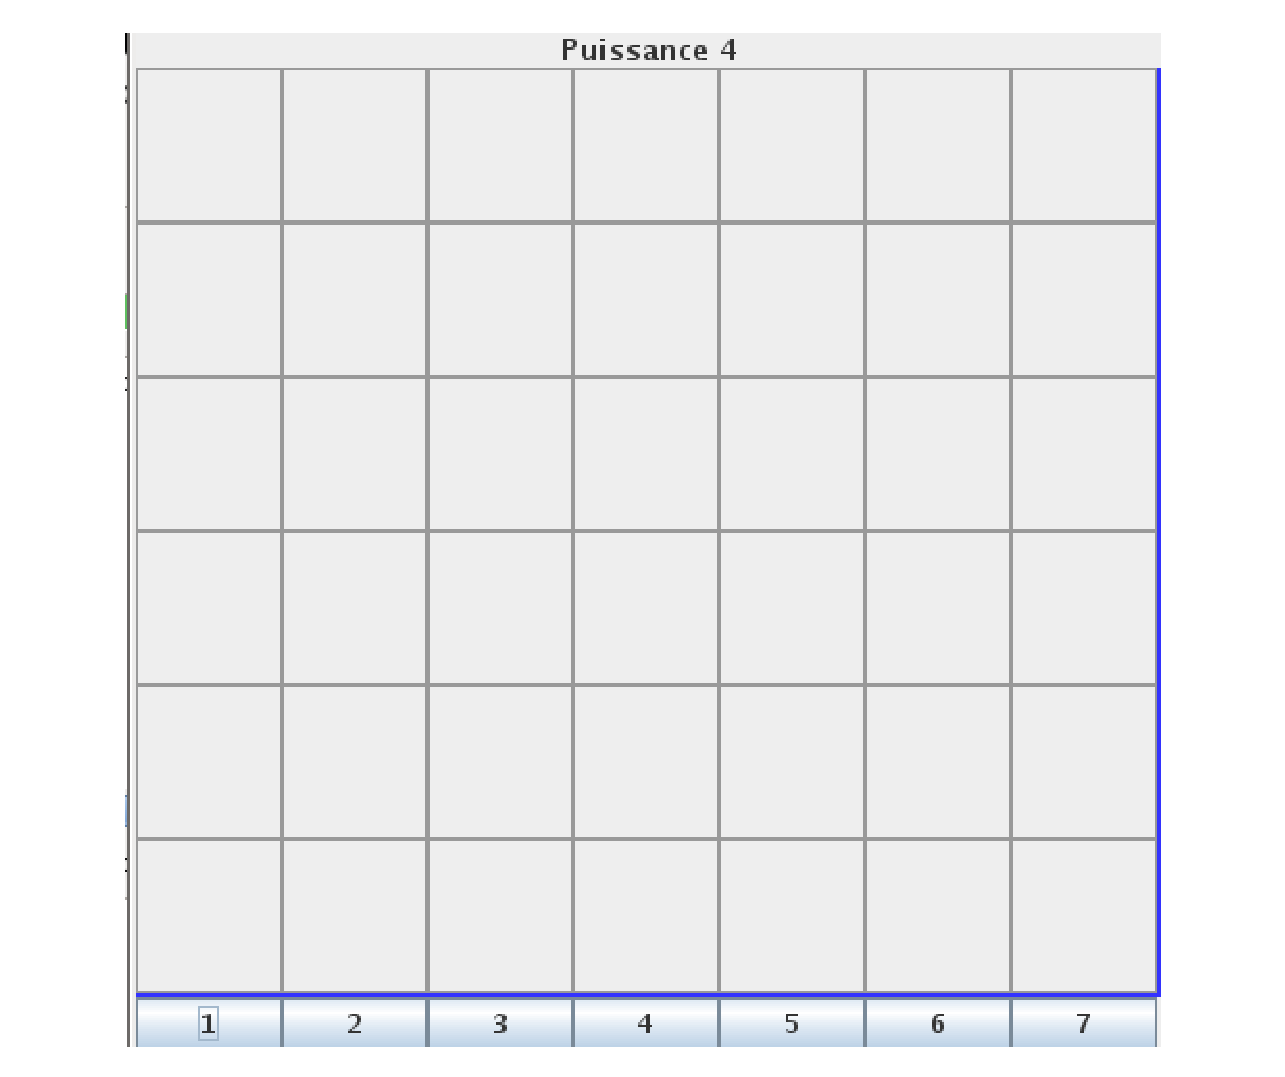
\includegraphics[scale=0.2]{nmfigempty}
  \caption{\texttt{Grille vide}}
\end{center}
\end{figure}

La grille est vide nous devons donc vérifier que l'ordinateur ne met pas encore en place de stratégie donc que 
\texttt{playable[]} est entièrement à 0 et que donc par défaut l'ordinateur joue au centre de la grille.


\begin{verbatim}
int Ia2Played = ia2.play(rule);
assertNotNull(Ia2Played);
assertTrue(0 <= Ia2Played && Ia2Played < grid.getWidth());
assertEquals(3, Ia2Played);
int[] playable2 = ia2.getPlayable();
for ( int i =0 ; i<ia2.getCpuGrid().getWidth();i++)
assertEquals(0,playable2[i]);
\end{verbatim}


\begin{figure}[H]
\begin{center}
  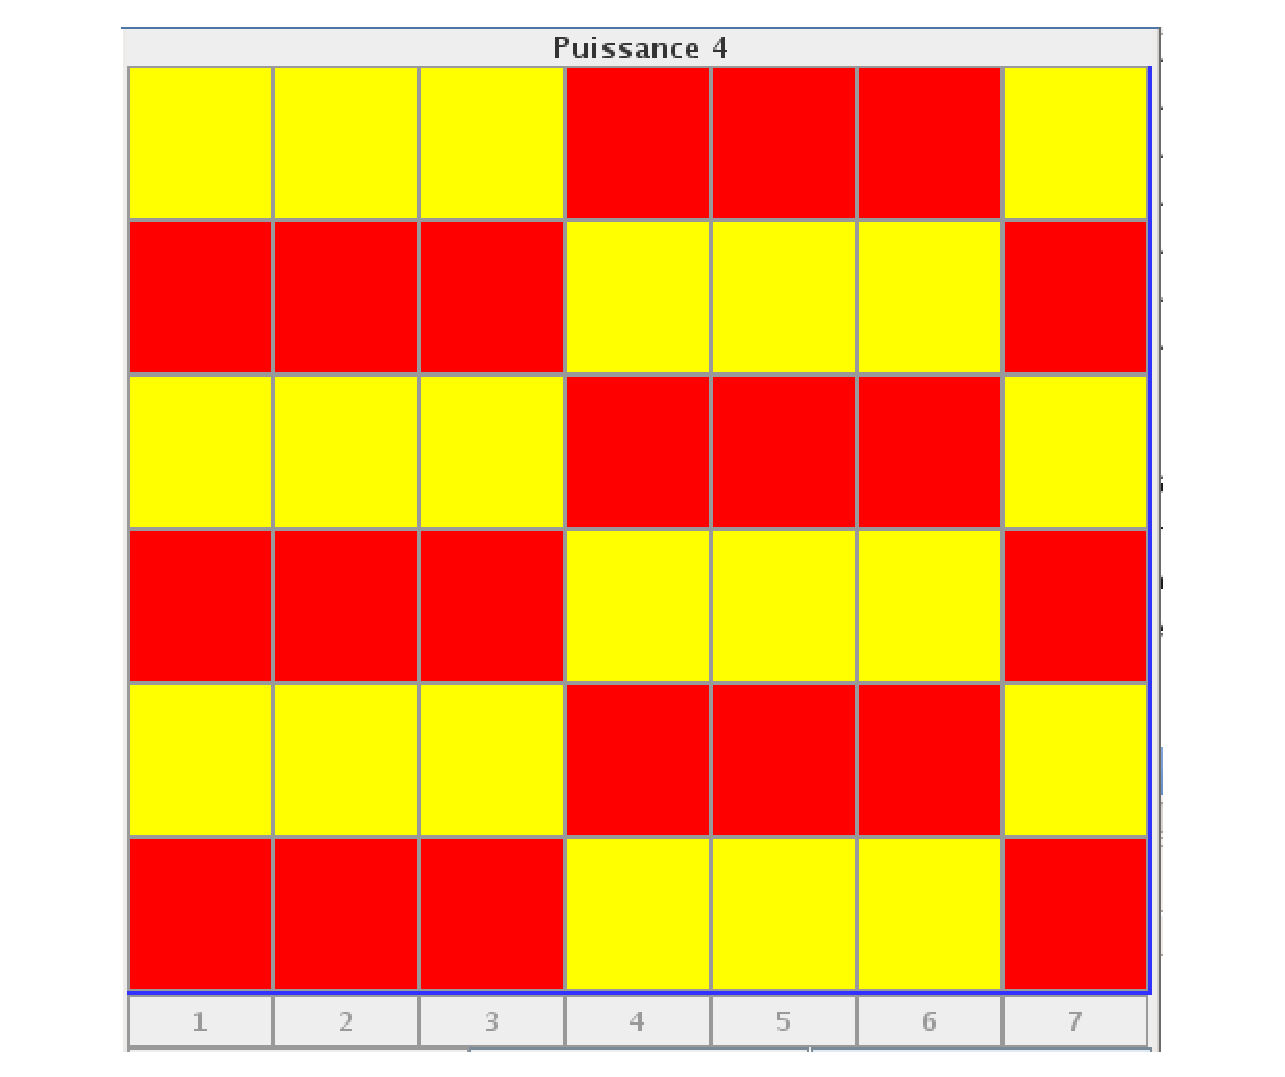
\includegraphics[scale=0.2]{nmfigfull}
  \caption{\texttt{Grille pleine}}
\end{center}
\end{figurre}

La grille étant pleine l'ordinateur ne peut donc pas jouer elle doit retourner le code d'erreur -1.

\begin{verbatim}
 int Ia2PlayedFullGrid = ia2.play(rule);
 assertFalse(0 <= Ia2PlayedFullGrid && Ia2PlayedFullGrid < grid.getWidth());
 assertEquals(-1, Ia2PlayedFullGrid);
\end{verbatim}

\begin{figure}[H]
\begin{center}
  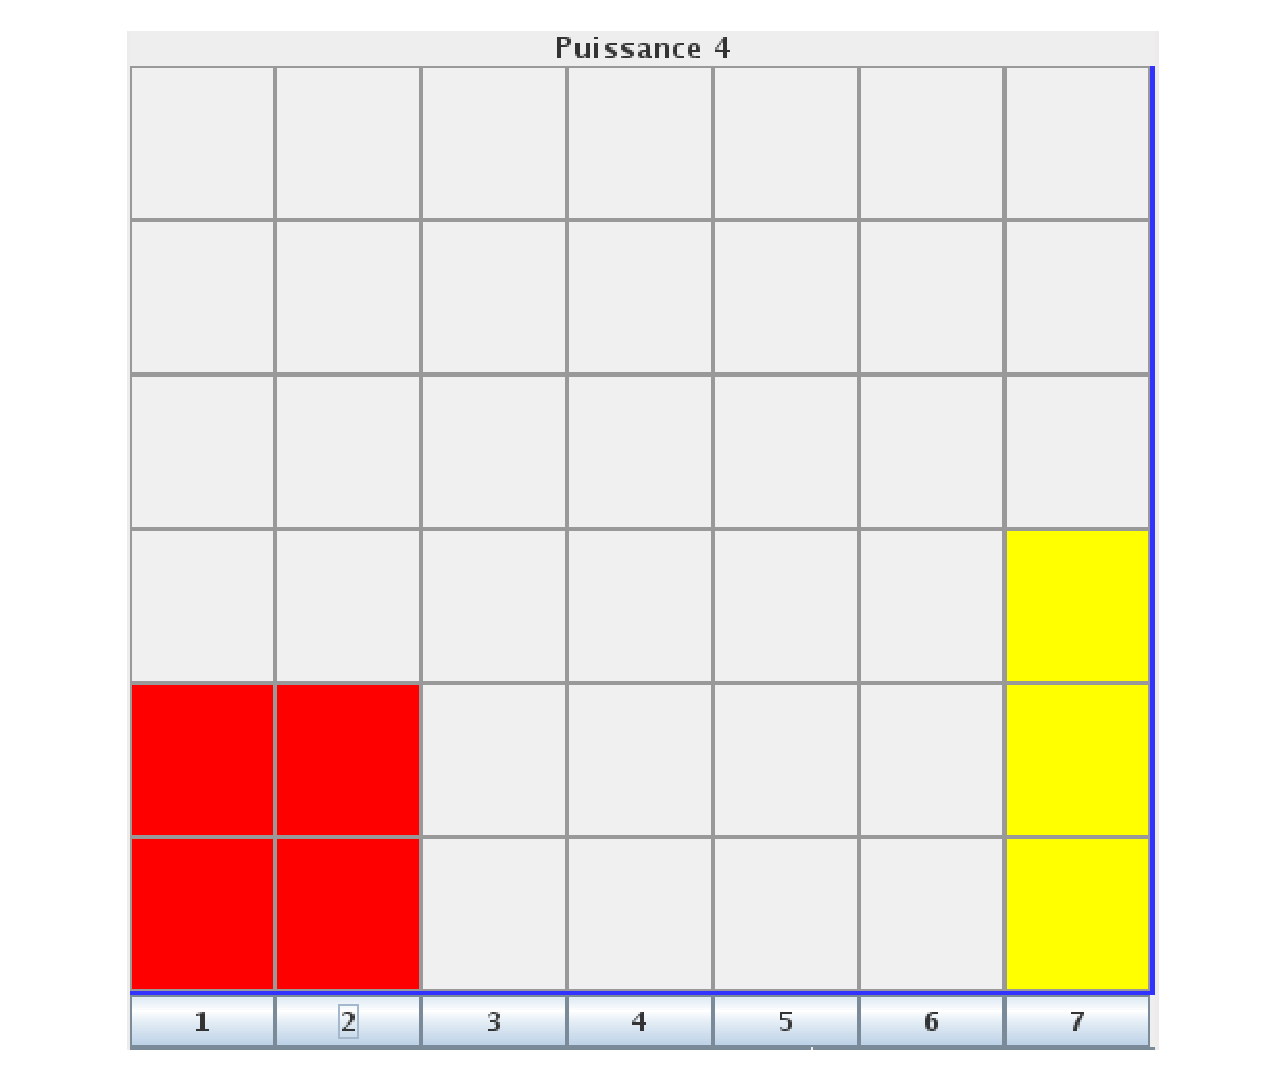
\includegraphics[scale=0.2]{nmfigwin}
  \caption{\texttt{Grille avec coup gagnant}}
\end{center}
\end{figurre}

Il y une la possibilité pour l'ordinateur de gagner, il doit donc repérer la colonne qui permet de gagner en y mettant le code \texttt{playable} à 3 et y jouer.

\begin{verbatim}
 int Ia4PlayedForWin = ia4.play(rule);
assertNotNull(Ia4PlayedForWin);
assertTrue(0 <= Ia4PlayedForWin && Ia4PlayedForWin < grid_null.getWidth());
assertEquals(6, Ia4PlayedForWin);
int[] playable4 = ia4.getPlayable();
for ( int i =0 ; i<ia4.getCpuGrid().getWidth();i++)
   if ( i == 6)
assertEquals(3,playable4[i]);
   else
assertEquals(0,playable4[i]);
\end{verbatim}


\begin{figure}[H]
\begin{center}
  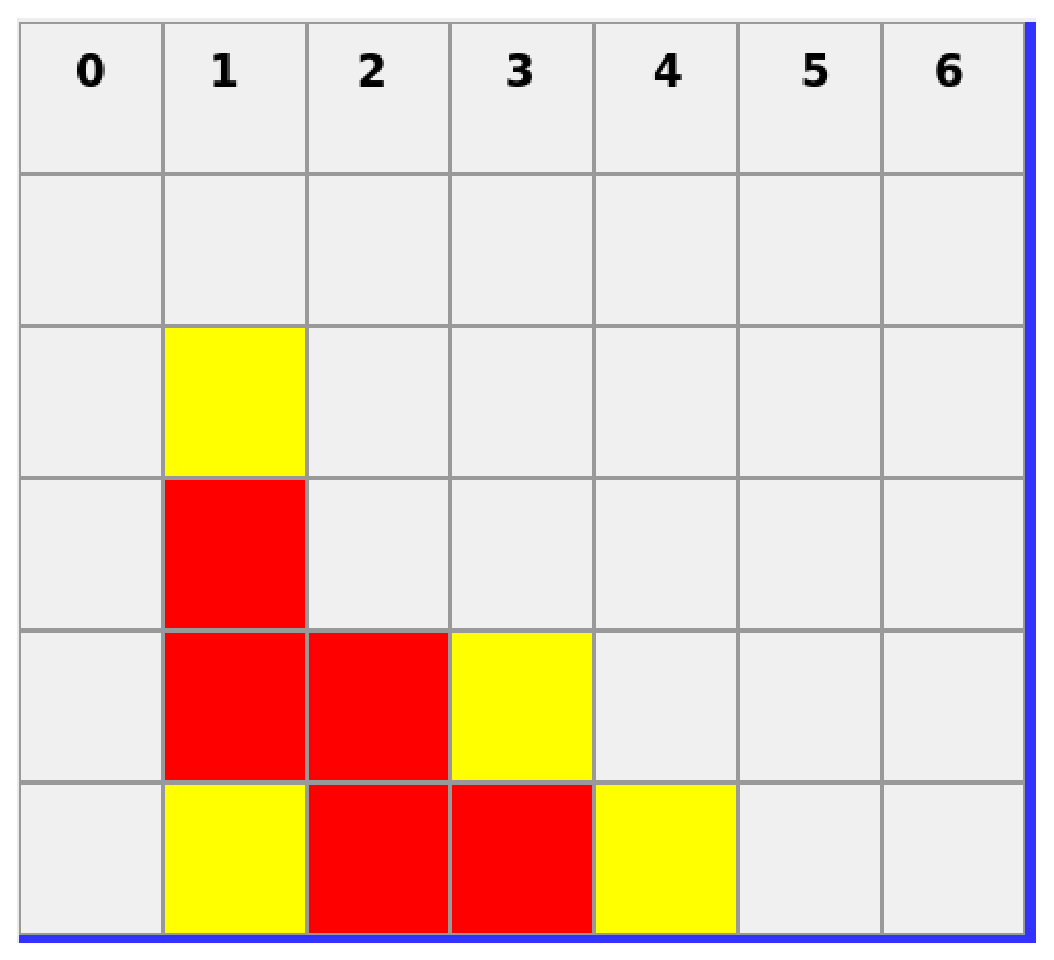
\includegraphics[scale=0.2]{playable3}
  \caption{\texttt{Autre cas de coup gagnant}}
\end{center}
\end{figure}

L'ordinateur peut à nouveau gagner en jouant en 2 et
donc il doit le faire avec \texttt{playable[2]=2}.

\begin{verbatim}
 int Ia2Playedfig4 = ia2.play(rule);
int[] playable7 = ia2.getPlayable();
assertEquals(2 , Ia2Playedfig4);
assertEquals(3, playable7[2]);
\end{verbatim}


\begin{figure}[H]
\begin{center}
  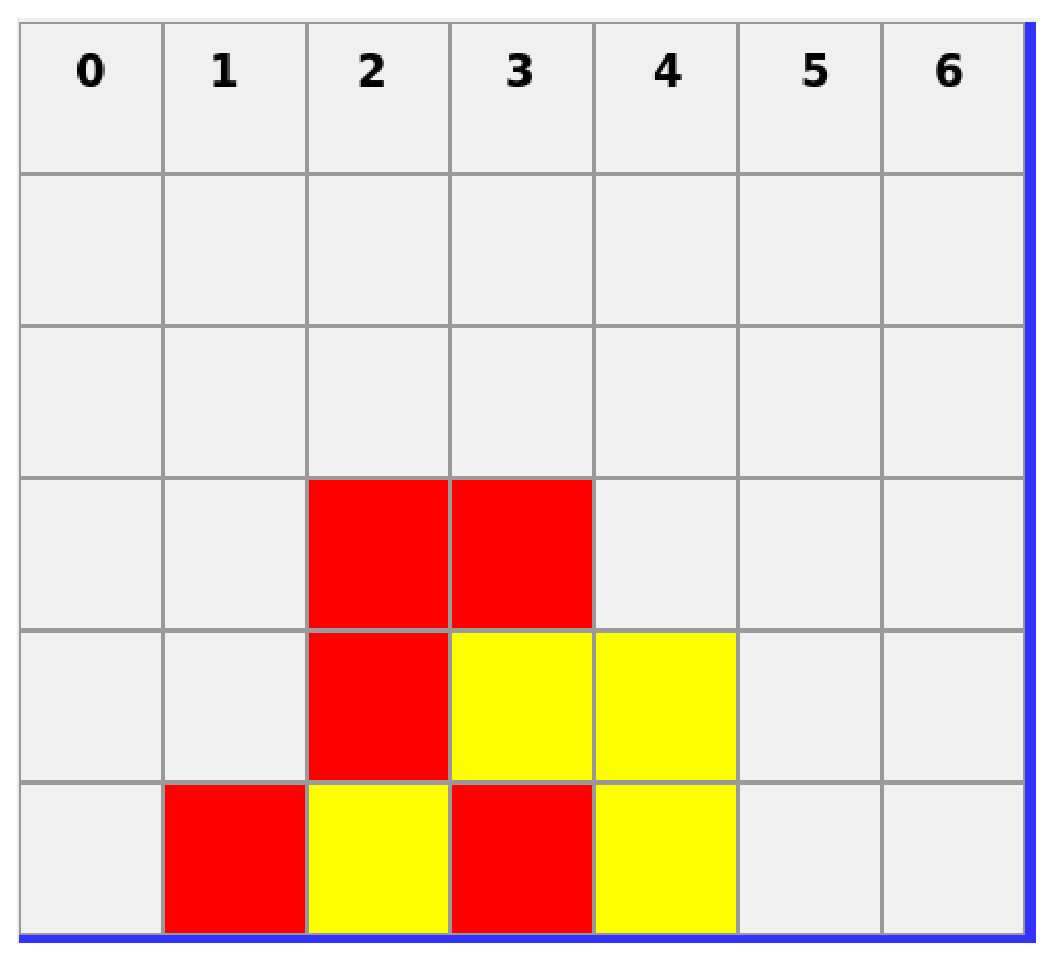
\includegraphics[scale=0.2]{playable10}
  \caption{\texttt{Colonne injouable}}
\end{center}
\end{figure}

Si l'ordinateur joue sur la colonne 4, alors au prochain coups l'autre joueur 
pourra gagner avec une diagonale. L'ordinateur devra donc avoir
\texttt{playable[4]=1} qui correspond a un placement de pions qui fait gagner l'adversaire
 et jouer sur une autre case, ici nous savons qu'il va jouer en 2
dut au fait du caractère non aléatoire de l'ordinateur.

\begin{verbatim}
 int Ia2Playedfig2 = ia2.play(rule);
int[] playable5 = ia2.getPlayable();
assertEquals(2 , Ia2Playedfig2);
assertEquals(1 , playable5[4]);
\end{verbatim}


\begin{figure}[H]
\begin{center}
  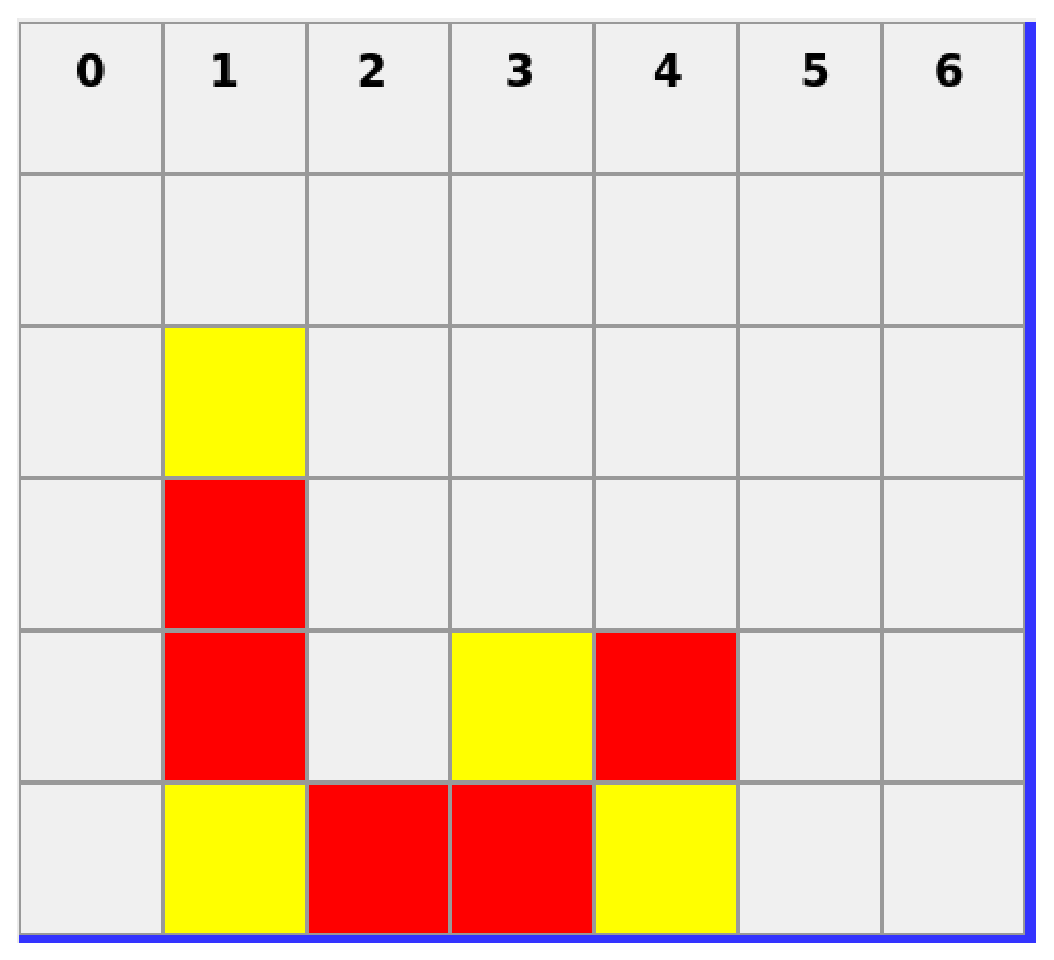
\includegraphics[scale=0.2]{playable2}
  \caption{\texttt{Stratégie sur plusieur coups}}
\end{center}
\end{figure}

Si l'ordinateur joue en 2 cela permettra a l'autre joueur de bloquer 
un éventuel coup gagnant futur.l'ordinateur doit avoir \texttt{playable[2] = 2} ce qui est
 un code moins fort que 1 mais il ne doit pas y jouer tout de même dans la mesure du possibles, si
il doit choisir entre un \texttt{playable} à 1 ou 2 il choisira tout de même le code 2.

\begin{verbatim}
 int Ia2Playedfig3 = ia2.play(rule);
int[] playable6 = ia2.getPlayable();
assertEquals(3 , Ia2Playedfig3);
assertEquals(2, playable6[2]);
\end{verbatim}




\begin{figure}[H]
\begin{center}
  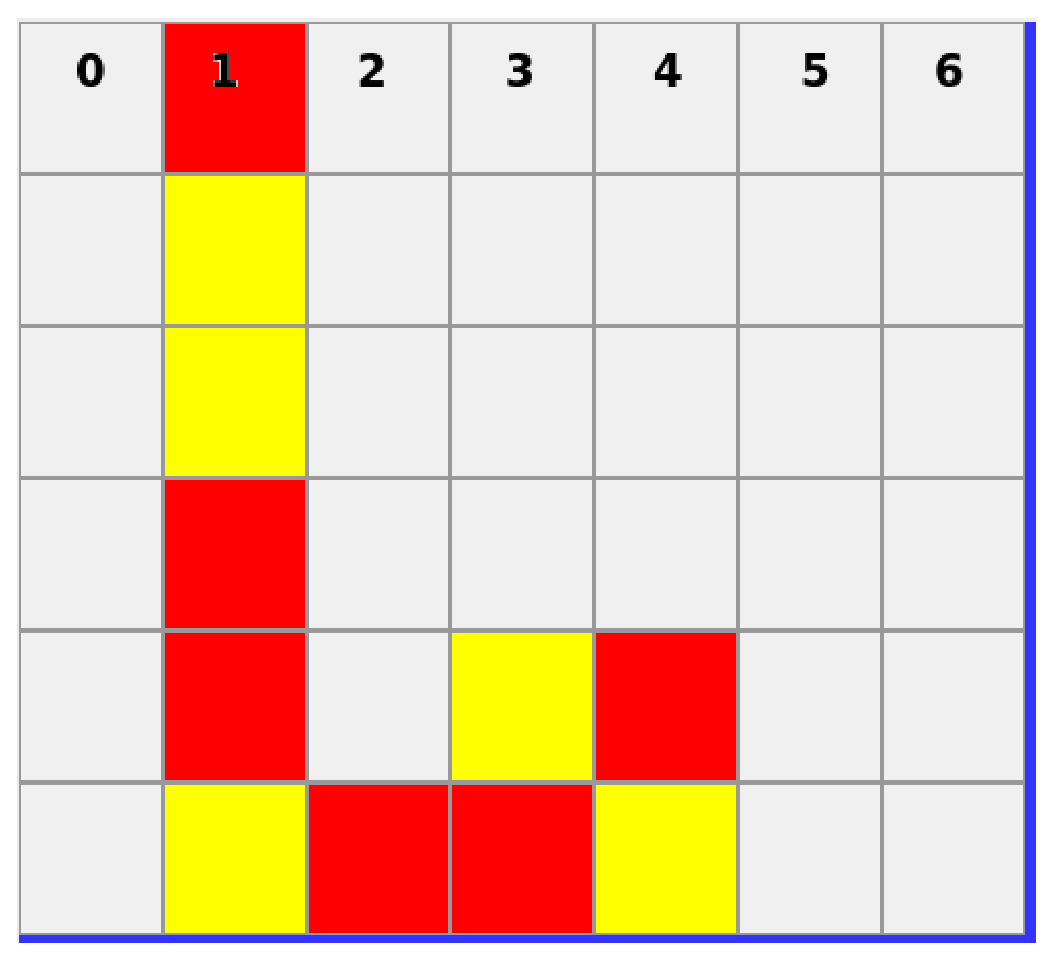
\includegraphics[scale=0.2]{playable4}
  \caption{\texttt{Colonne injouable}}
\end{center}
\end{figure}

La colonne 1 est pleine donc l'ordinateur ne doit plus y jouer et  \texttt{playable[1] = 4}.
C'est le code qui interdit de jouer le plus fort si tout les colonnes sont a 4 il renvera un code d'erreur -1.
C'est le seul code de \texttt{playable}  ou il est totalement impossible de jouer dans la colonne marqué.


\begin{verbatim}
 int[] playable8 = ia2.getPlayable();
assertEquals(4, playable8[1]);
\end{verbatim}


\begin{figure}[H]
\begin{center}
  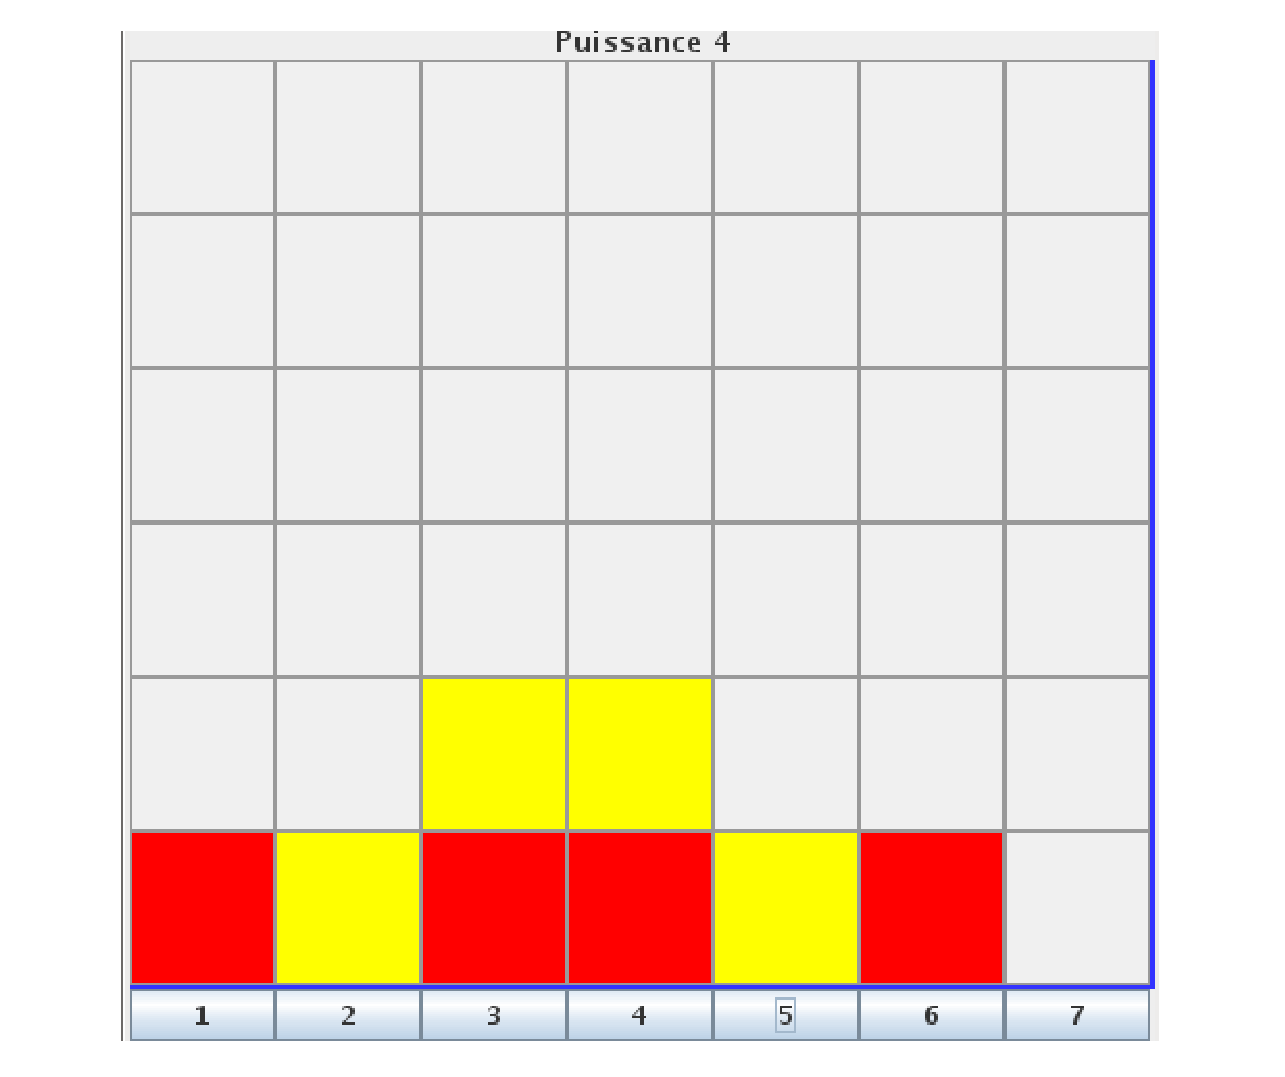
\includegraphics[scale=0.2]{nmfig6}
  \caption{\texttt{Strategie sur plusieurs coup}
\end{center}
\end{figure}

L'ordinateur doit remarquer qu'il peut gagner en deux coup il met donc \texttt{playable}
à 5 sur les cases offrant cette possibilité : \texttt{playable[2] =  5} et \texttt{playable[5] = 5}.
(  colonne 2 et 6 sur la grille ).Il prépare donc comme voulu sa stratégie sur 2 coups qu'il modifiera en 
fonction de du coup jouer par l'autre joueur.

\begin{verbatim}
 int Ia2Playedfig6 = ia2.play(rule);
int[] playable9 = ia2.getPlayable();
assertEquals(5 , Ia2Playedfig6);
assertEquals(5, playable9[1]);
assertEquals(5, playable9[5]);
\end{verbatim}


\begin{figure}[H]
\begin{center}
  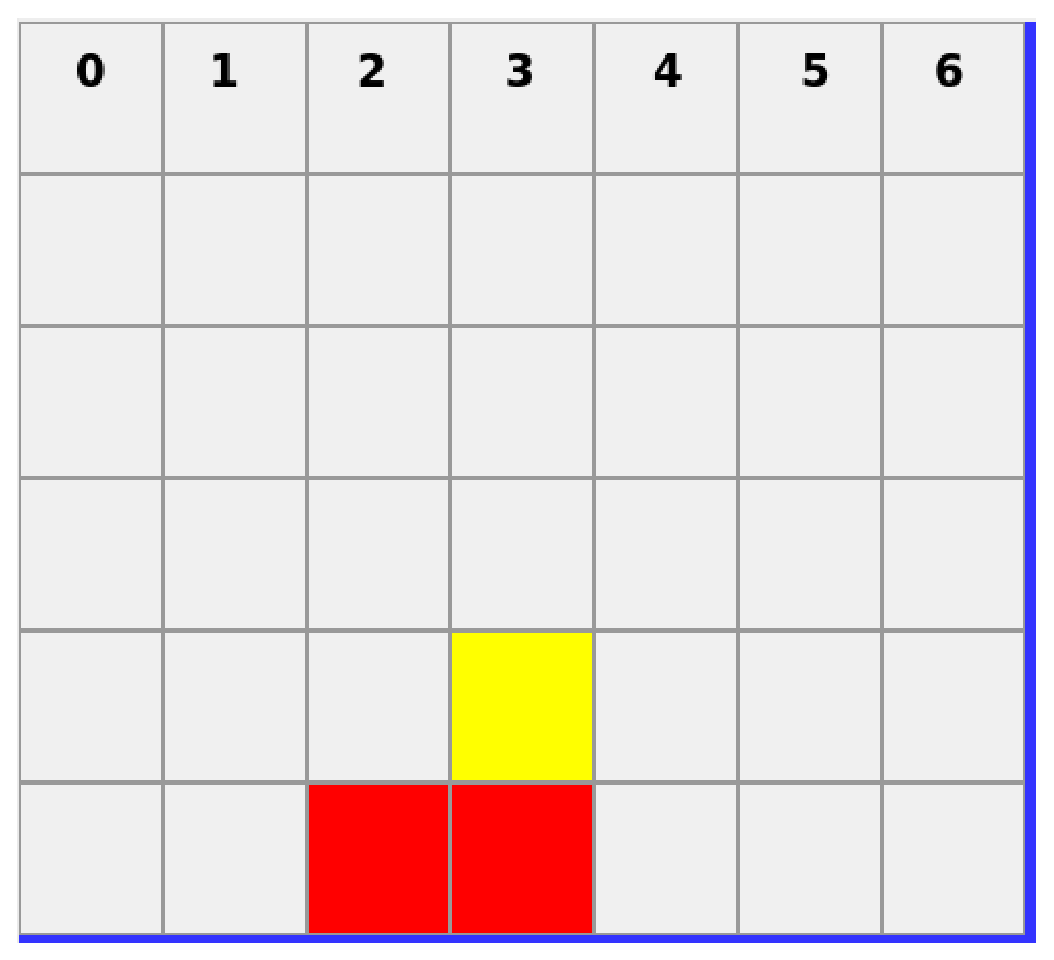
\includegraphics[scale=0.2]{playable1}
  \caption{\texttt{Stratégie de blocage}}
\end{center}
\end{figure}
L'ordinateur peut aussi prévoir à l'avance les positions dangereuses des pions de l'autre joueur,
il mettra ainsi en place la tactique \texttt{playable} 6 dans les colonnes qui couperont les alignements 
possibles des pions adverses.Dans ce cas la \texttt{playable[1] = 6} et \texttt{playable[4] = 6}.Il jouera donc dans
l'une de ces deux colonnes , ici la colonne 4.

\begin{verbatim}
int Ia2Playedfig7 = ia2.play(rule);
int[] playable10 = ia2.getPlayable();
assertEquals(4 , Ia2Playedfig7);
assertEquals(6, playable10[0]);
assertEquals(6, playable10[4]);
\end{verbatim}


\begin{figure}[H]
\begin{center}
  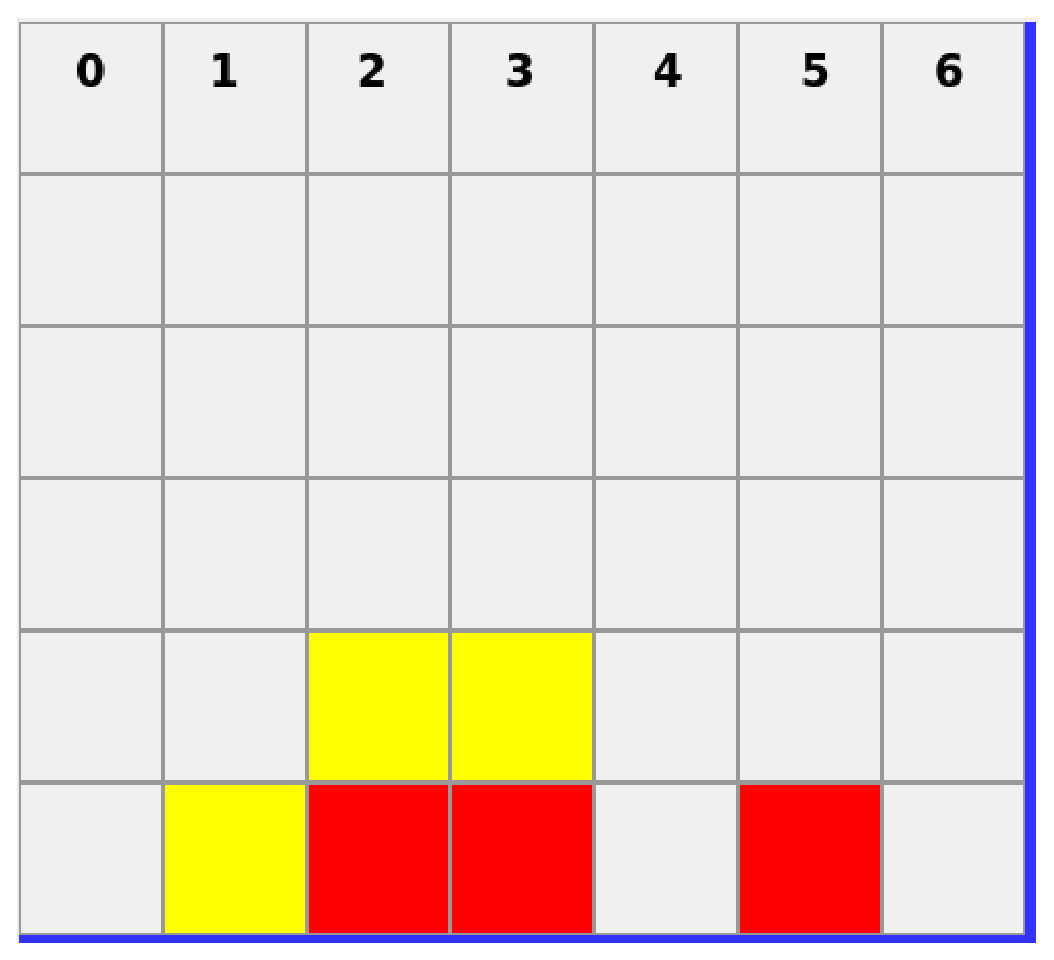
\includegraphics[scale=0.2]{playable6}
  \caption{\texttt{Coup Obligatoire}}
\end{center}
\end{figure}

L'ordinateur est obliger de jouer en colonne 4 sous peine de voir l'autre joueur gagner au prochain coup.
Nous devons donc avoir \texttt{playable[4]=6} qui est le code prioritaire pour les coups à jouer. 

\begin{verbatim}
 int Ia2Playedfig8 = ia2.play(rule);
int[] playablefig8 = ia2.getPlayable();
assertEquals(4 , Ia2Playedfig8);
assertEquals(6, playablefig8[4]);
\end{verbatim}


\begin{figure}[H]
\begin{center}
  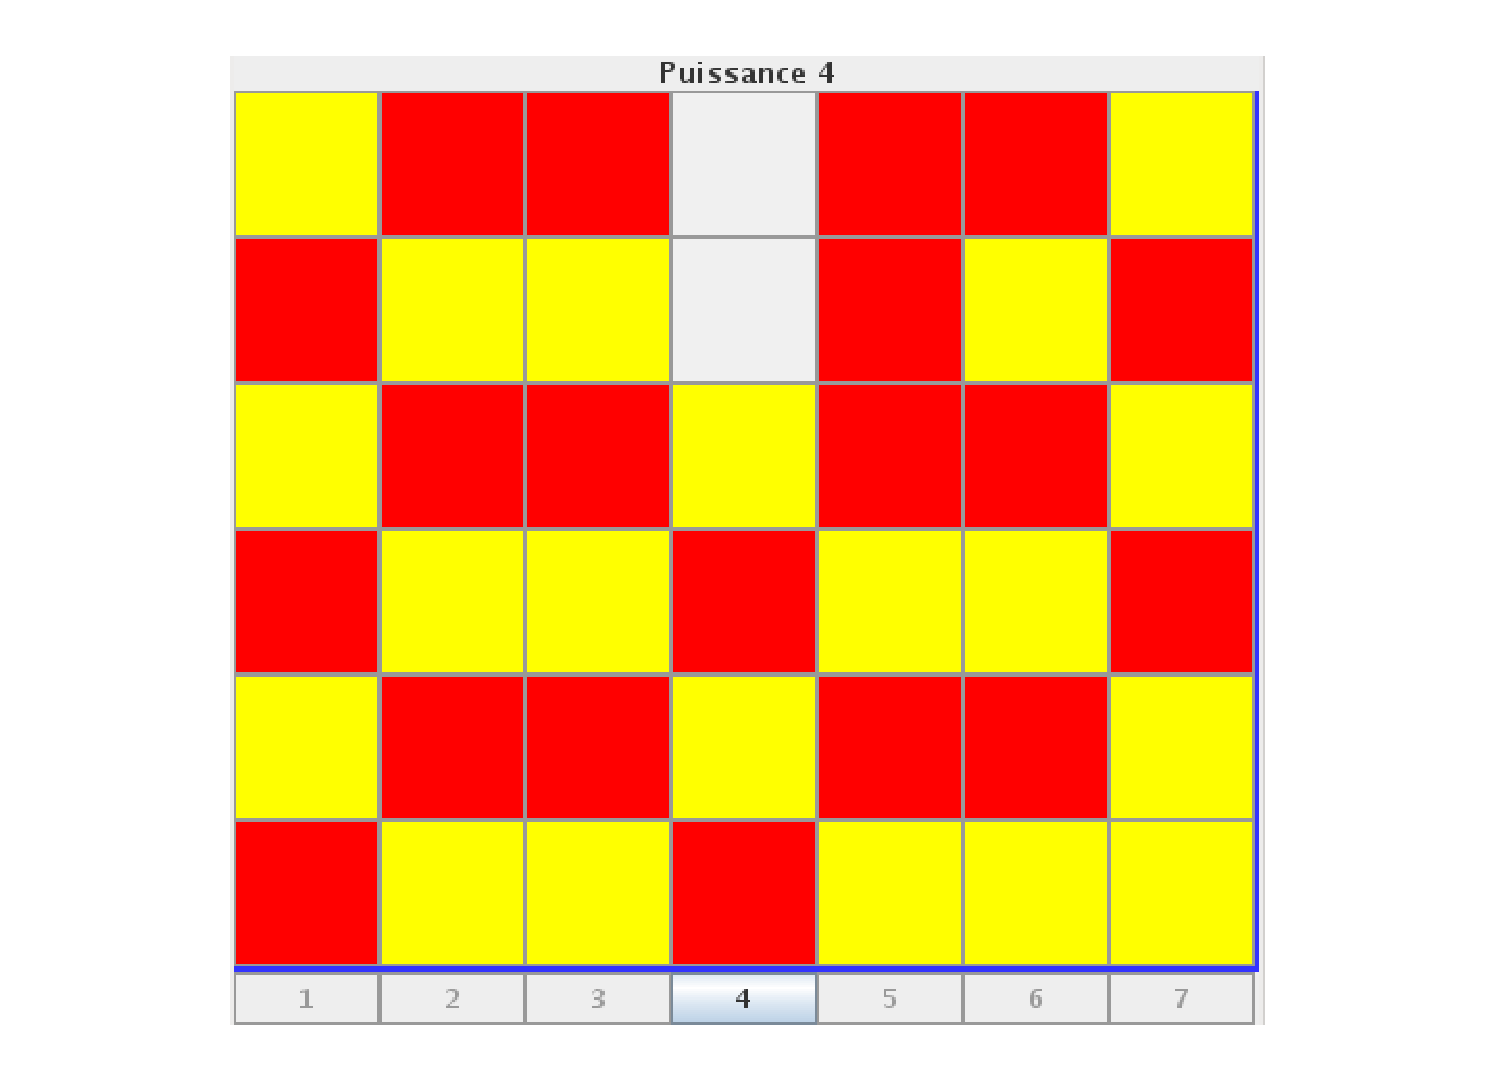
\includegraphics[scale=0.2]{nmfig9}
  \caption{\texttt{Non blocage du jeu}}
\end{center}
\end{figure}
Il peut arriver que l'ordinateur n'est pas le choix et doit jouer dans une colonne même si son
\texttt{playble} est à 1  c'est a dire que jouer ce coup fera gagner l'autre joueur, nous devons vérifier que l'ordinateur le fera quand même sous peine de bloquer la partie.Donc ici \texttt{played[3]=1} , mais l'ordinateur joue en 3 (4ème colonne) et fait ainsi gagner l'autre joueur.

%%%%%%%%bug%%%%%%%%

Ces tests nous ont permis de révéler de nombreux bugs liée aux comportements des IA. Tout d'abord sur les stratégies de \texttt{playable[]) qui n'était pas toujours juste par rapport à l'état actuel de la grille,et aussi le façon de jouer des IA ne correspondait pas toujours à ce qui était attendut dut au fait des priorités des \texttt{playable}.

Pour chaque état de la grille il nous était possible a l'aide de l'algorithme de connaitre l'état de \texttt{playable[]} et le coup que doit jouer l'IA ainsi nous avons corriger les moteurs d'IA pour qu'ils nous donnes exactement les résultats escomptés dans les cas typiques ci-dessus.

%%%%%%%cfa%%%%%%

